%!TEX root = report.tex
This chapter discusses the front-end. We start by presenting the technology stack in \cref{sec:1:technologyStack}. After that we describe the most important control flows in the front-end in the section \nameref{sec:1:design}.

\section{Technology Stack}
\label{sec:1:technologyStack}
	This section devotes on section to each technology on the front-ends stack. For each technology we will describe what it does and why we opted to use this technology in favour of other options.

	\subsection{AngularJS}
	\label{ssec:1:angularjs}
		% What is it
		AngularJS is a web application framework by Google for creating dynamic web applications. 

		AngularJS depends on JQuery, thus we had to include that to. We have also used JQuery in some places for the removing and adding of classes where to resulted in neater code than using Angular directives.\\

		% Why have we used this technology, mention alternatives
		We chose to use AngularJS since one of us had some experience with it. We considered Backbone as an alternative but dropped it for its flexibility, which may be great if you are an experiences web developer and know exactly what you want, but would have been too much for us. Furthermore it is advised to add a framework on top Backbone which would have added to the learning curve for Backbone \cite{AComparisonofAngularBackboneCanJSandEmber}. 

		Apart from the previous experience the fact that AngularJS was specifically developed for single page applications is what made us decide in favour of AngularjS.\\

		% Would we make the same choice again?
		One of the downsides of AngularJS is that its learning curve, after learning the basic features is quite steep. The documentation is rife with Angular-specific terms which makes it hard to read.

		\subsubsection*{Extensions}
		We have used some extensions to Angular. We list them and shortly describe their functionality.

			\begin{description}
				\item[ngRoute] provides routing and deep-linking services and directives for angular applications \cite{angulardocsngRoute}. We use it to make it possible to store a link to a specific part of our application. 
				\item[ngFacebook] provides an interface between AngularJS and the Facebook API. We have adapted the source of this service in some places to make it better suited to our purposes and to keep it consistent with \t{ngLinkedIn}.
				\item[ngLinkedIn] is for LinkedIn what \t{ngFacebook} is for Facebook. We have also adapted its source code to extend its functionality and to keep it consistent with \t{ngFacebook}.
				\item[angular-md5] is a service that computes MD5 hashes. We use it to hash the Facebook and LinkedIn identifier of our users, so that we can find multiple searches of one user without storing the actual user. 
				% \item[angular-http-loader] %we don't seem to use it?ng.httpLoader
			\end{description}

	\subsection{Bootstrap}
	\label{ssec:1:bootstrap}
		% What is it
		Bootstrap is a framework by Twitter which places emphasis on responsive design. 

		% Why have we used, mention alternatives
		Although there are alternatives to Boostrap, i.e. Zimit, InK or Pure, we did not really consider them since we were both familiar with Bootstrap and felt that we had enough new technologies to worry about. We did however use a different theme from \url{http://bootswatch.com} to avoid the distinctive Bootstrap look and feel. We add Font Awesome for the icons it provides. 

	\subsection{UI Bootstrap}
	\label{ssec:1:bootstrapUI}
		UI Bootstrap is an Angular version of the JavaScript part of Bootstrap. As far as we could find there are no alternatives other than building the directives yourself. 

		In the end we had to write the carousel at the login window, see \vref{fig:1:viewLogIn}, ourselves since the custom buttons we wanted were not supported by UI Bootstrap.

	\subsection{Dangle}
	\label{ssec:1:dangle}
		% What is it
		``Dangle is a set of AngularJS directives that provide common visualizations based on D3."\cite{dangle}

		% Why have we used it, mention alternatives
		We have used it to create the pie charts shown on the statistics page, after practically rewriting the directive. The directives provided by Dangle did not handle long labels, and pie charts with a lot of pieces very well. To solve this we have removed all code from the pie chart directive that added labels and added a separate legend, see \vref{fig:1:viewStat}. The one upside of Dangle was that it expected its input in the same format our map-reduce-operations returned it. \\

		% Would we make the same choice again?
		In hindsight we should have chosen something other than Dangle, however we did not look further since Dangle played nice with AngularJS. 

	\subsection{RequireJS}
	\label{ssec:1:requirejs}
		% What is it
		RequireJS is a JavaScript file and module loader that is optimized for in-browser use. Neither one of us had any experience with anything like it and since RequireJS was mentioned during the lectures we chose to use it. It helped that we found a boilerplate project that combined AngularJS and RequireJS. \todo{Where did we get the boilerplate?}	

\section{Design}
\label{sec:1:design}
	In this section we will discuss the control flow in the front end upon certain actions of the user. To avoid a lengthy report we will only discuss the flow of successful cases.

	\subsection{Log In}
		As mentioned earlier users have to log in to a social network before being allowed to stalk somebody on that network. Since we store the ID of the user and we have not implemented an api call that adds for example the LinkedIn identification to a user that we have already stored with its Facebook identification.

		\Cref{fig:1:controlflowLogIn} presents the flow of control when a users logs in. The views that are presented to the user before and after logging in are presented in \cref{fig:1:viewLogIn}.

		The \t{loggedIn}, and its not shown equivalent \t{loggedOut}, event ensure that the \t{searchController} knows that a user is logged in. The \t{Facebook Service}, \t{ngFacebook}, is discussed \vref{ssec:1:angularjs}.

		\begin{figure}
			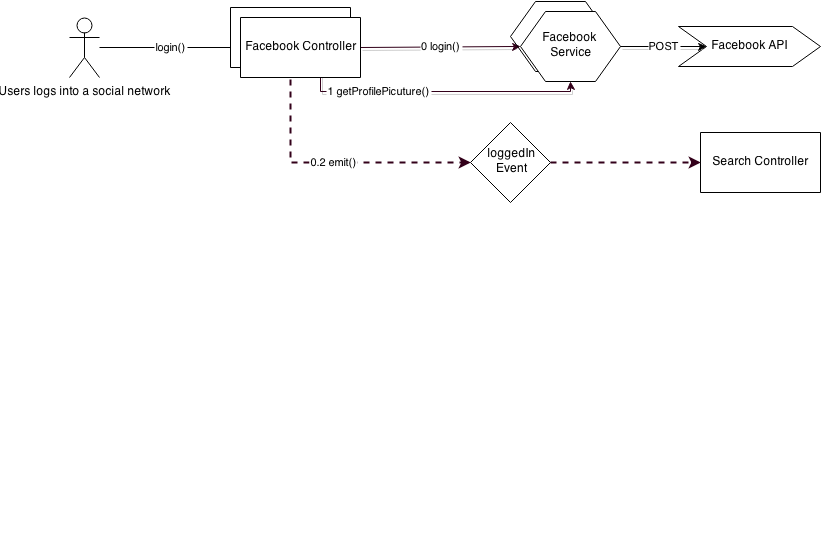
\includegraphics[width=\textwidth]{./img/1_login_flow}
			\caption{A schematic overview of the control flow when a user logs in.}
			\label{fig:1:controlflowLogIn}
		\end{figure}

		\begin{figure}
			\begin{subfigure}{\textwidth}
				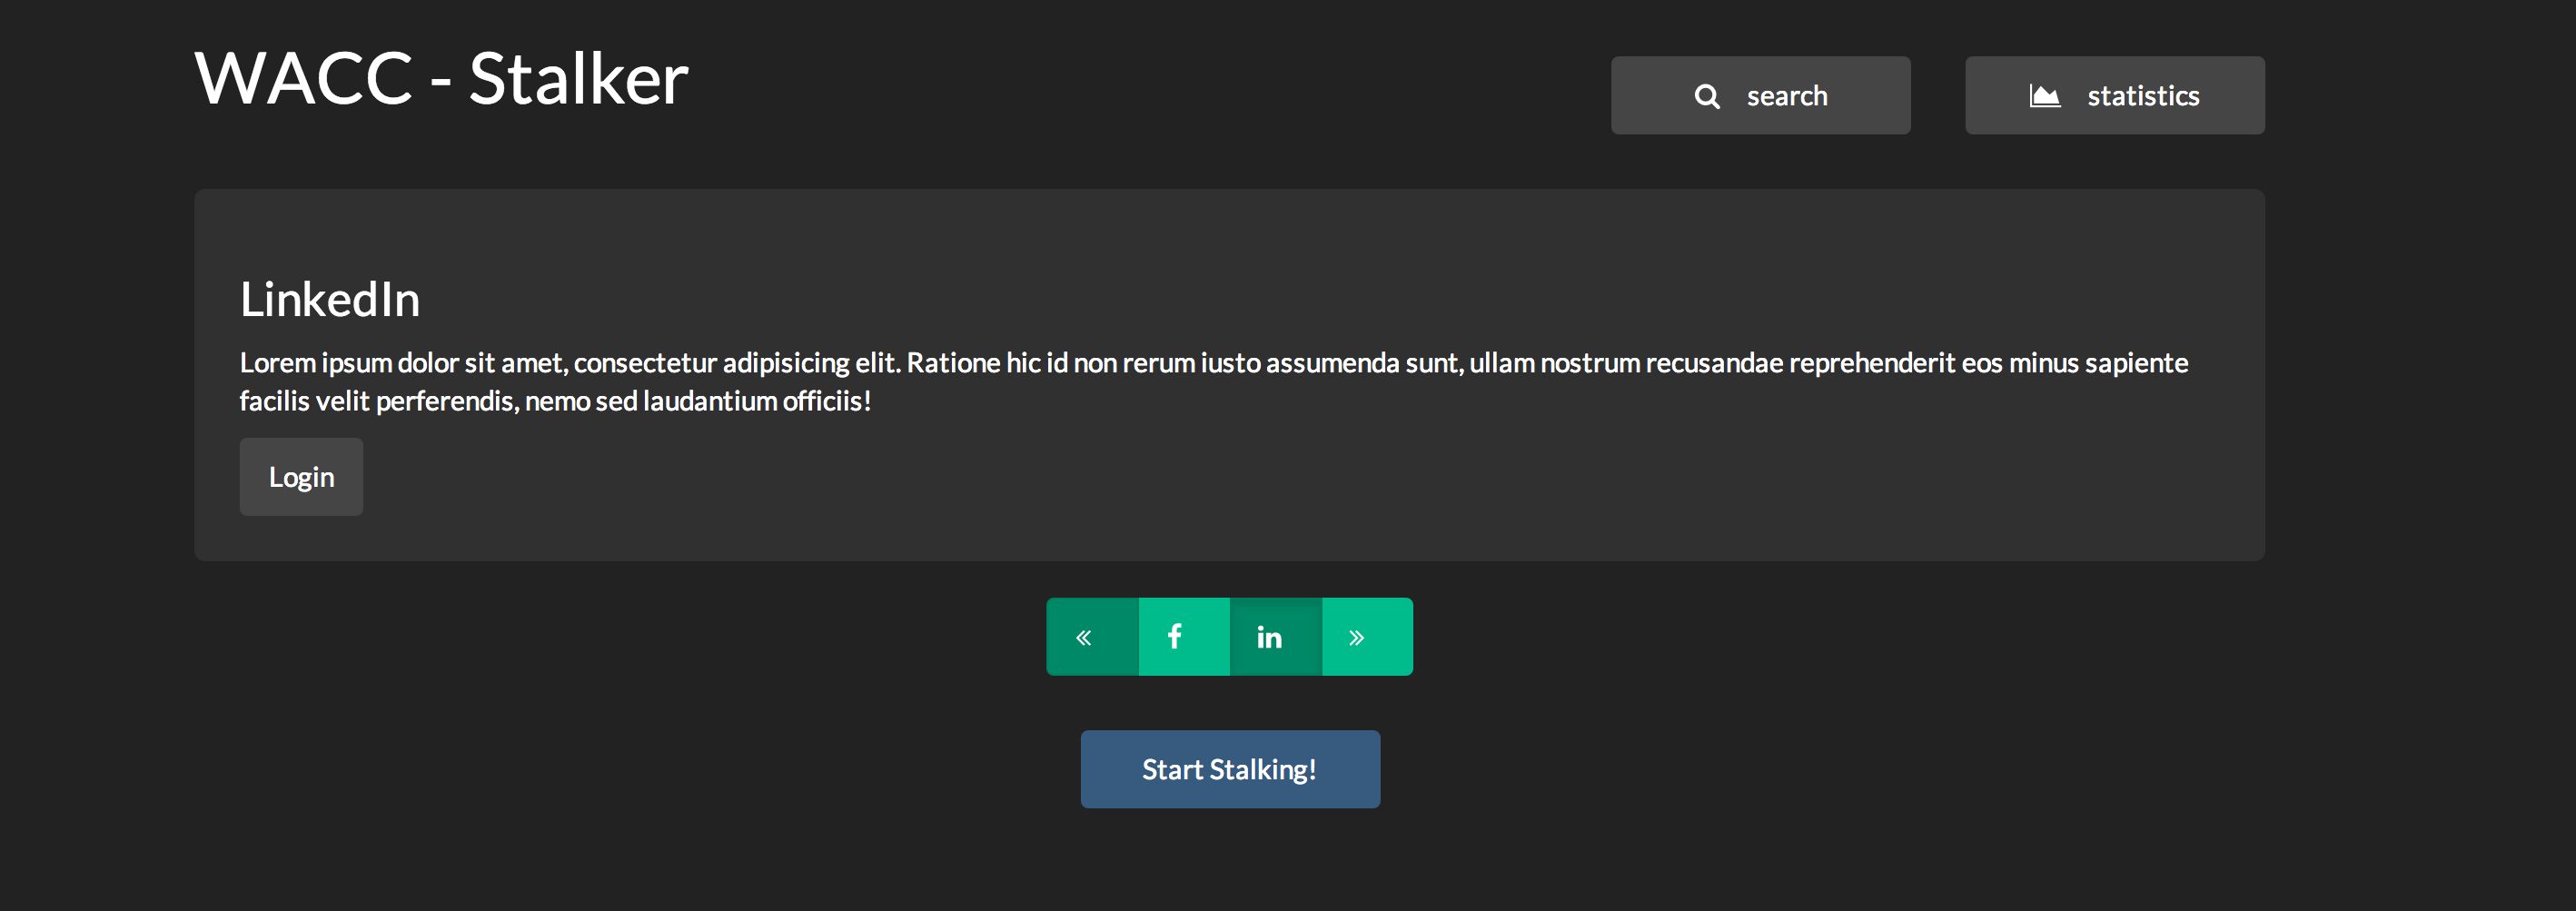
\includegraphics[width=\textwidth]{./img/1_login_view_logged_out}
				\caption{The view when the user is not logged into LinkedIn.}
				\label{fig:1:viewLogIn:linkedin}
			\end{subfigure}
			\begin{subfigure}{\textwidth}
				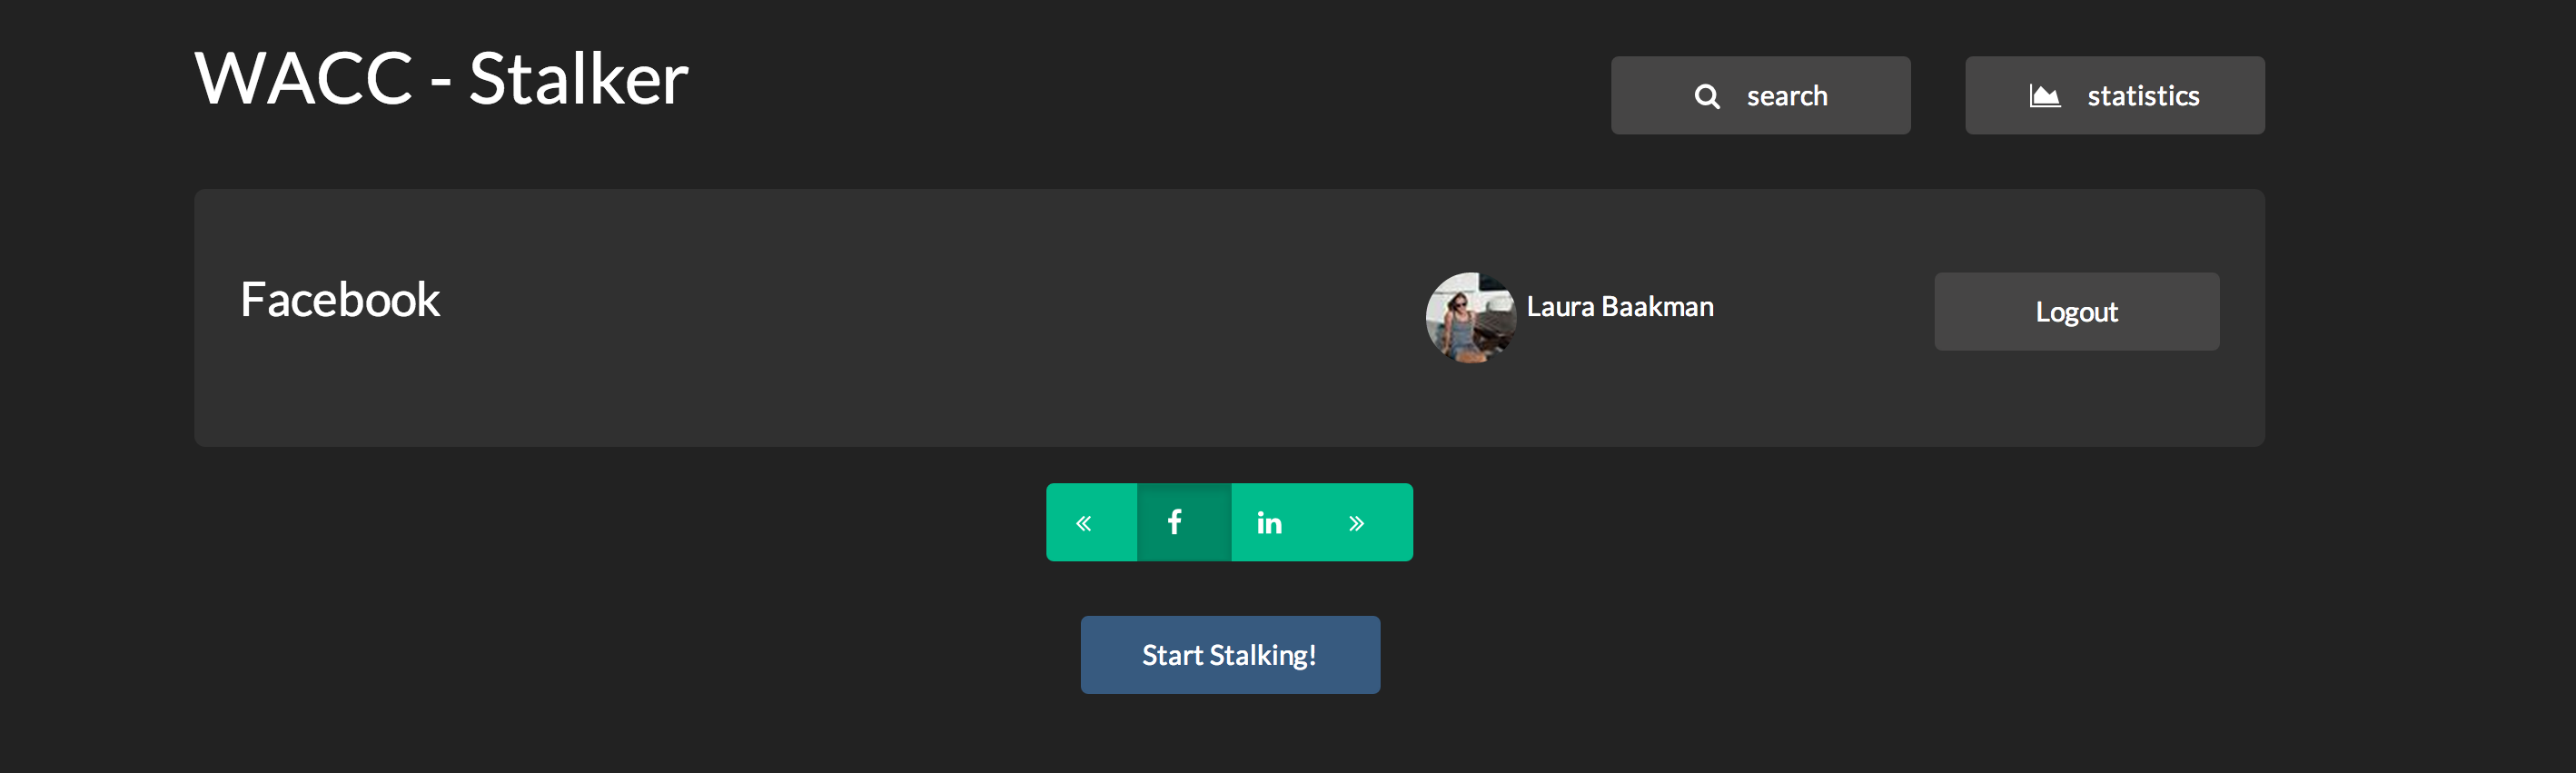
\includegraphics[width=\textwidth]{./img/1_login_view_logged_in}
				\caption{The view when the user is logged into Facebook.}
				\label{fig:1:viewLogIn:facebook}
			\end{subfigure}			
			\caption{Screen shots of the application when \subref{fig:1:viewLogIn:facebook} the user still has not yet logged into LinkedIn and \subref{fig:1:viewLogIn:linkedin} the user has logged in into Facebook.}
			\label{fig:1:viewLogIn}
		\end{figure}	

	\subsection{Log Out}	
			The control flow when a user logs out is presented in \cref{fig:1:controlflowLogOut}. 
			\todo{Begeleidend verhaaltje schrijven.}	

			\begin{figure}
				\missingfigure{Control flow of logging out}
				\caption{A schematic overview of the control flow when a user logs out.}
				\label{fig:1:controlflowLogOut}
			\end{figure}		

	\subsection{Stalk}
		\Cref{fig:1:controlflowStalk} presents the flow of control when a user searches for somebody on the social networks that he has logged in to. The views presented to the user are shown in \autoref{fig:1:viewStalk}.

		\todo{Begeleidend verhaaltje schrijven}

			\begin{figure}
				\missingfigure{Control flow of stalking}
				\caption{A schematic overview of the control flow when a user stalks somebody.}
				\label{fig:1:controlflowStalk}
			\end{figure}	

			\begin{figure}
				\begin{subfigure}{\textwidth}
					\missingfigure{Screenshot of the application when a user has to start filled out data, and is about to press the stalk button.}
					\caption{The view when the user is about to press the stalk button.}
					\label{fig:1:viewStalk:startStalk}
				\end{subfigure}
				\begin{subfigure}{\textwidth}
					\missingfigure{Screenshot with a list of results.}	
					\caption{The view when all victims are found.}
					\label{fig:1:viewStalk:allVictims}
				\end{subfigure}		
				\begin{subfigure}{\textwidth}
					\missingfigure{Screenshot with a one result}	
					\caption{The view with the details of one victim.}
					\label{fig:1:viewStalk:oneVictim}
				\end{subfigure}						
				
				\caption{Screen shots of the application when \subref{fig:1:viewStalk:startStalk} the user is about to press the stalk button, \subref{fig:1:viewStalk:allVictims} the list of all victims, \subref{fig:1:viewStalk:oneVictim} the details of one victim.}
				\label{fig:1:viewStalk}
			\end{figure}

	\subsection{View Statistics}
		The control flow when a user views statistics is presented in \cref{fig:1:controlflowStat}. \Cref{fig:1:viewStat} shows how the statistics are presented to the user.

		\todo{Begeidend verhaaltje schrijven}

		\begin{figure}
			\missingfigure{Control flow of statistics}
			\caption{A schematic overview of the control flow of requesting the statistics and showing them to the user.}
			\label{fig:1:controlflowStat}
		\end{figure}

		\begin{figure}
			\missingfigure{View statistics}
			\caption{The view when the user has requested statistics.}
			\label{fig:1:viewStat}
		\end{figure}